\chapter{}
Wiederholung was ist eine Basis einer Topologie?
\dfn{Basis einer Topologie}
{
    Sei $(X, \mathcal{T})$ ein topologischer Raum. Eine Menge 
    $\mathcal{B} \subseteq \mathcal{T}$ heißt \textbf{Basis} der Topologie 
    $\mathcal{T}$, wenn für jedes $O \in \mathcal{T}$ eine Teilmenge 
    $\mathcal{B}_O \subseteq \mathcal{B}$ existiert, so dass
    $$
        O = \bigcup_{B \in \mathcal{B}_O} B .
    $$
}
Die Frage konnte sich mein imaginärer Läser jetzt sehr schnell durch 
weiterlesen beantworten.\\
Ein andere Frage die ich mir stelle ist:\\
Die Vorlesungsprüfung umfasst den Stoff der Vorlesung jedoch zb, 
der Begriff der Basis wurde in der Übung eingeführt.
Wäre die Basis nicht wiederholt worden, wäre sie dann prüfungsrelevant?



Aber naje $\dots$ Weiter mit Stoff:
Zur einleitung ein äher Kreifbares Beispiel.

\ex{}
{Sei $(X, \mathcal{T})$ ein Metrischer Raum.
Und $\mathcal{T}_d$ die von der Metrik induzierte Topologie.
Dann ist $$
\mathcal{B} = \{ U_{\frac{1}{n}}(x) : x \in X, n \in \mathbb{N} \}
$$
eine Basis der Topologie $\mathcal{T}_d$.
}

\dfn{Subbasis}
{
    Sei $(X, \mathcal{T})$ ein topologischer Raum. Eine Menge 
    $\mathcal{S} \subseteq \mathcal{P}(X)$ heißt \textbf{Subbasis} 
    der Topologie 
    $$
    : \Leftrightarrow \mathcal{T}
    \text{ ist die kleineste Topologie,
     die } \mathcal{S} \text{ umfasst. }
    $$
}

\begin{figure}[h!]
 \centering
    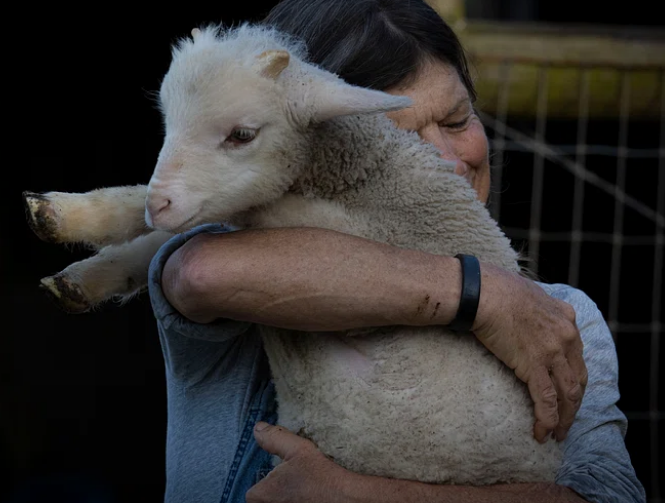
\includegraphics[width=0.6\textwidth]{pictures/hug_lemma.png}
    \caption{\url{https://creativecommons.org/licenses/by-nd/4.0/}\\
    Mensch Umfasst Lamm (Lemmachen).\\
    Wäre der Mensch die kleinste Topologie, 
    die das Lamm umfasst,\\
    so wäre der Mensch eine Subbasis.$\dots$ missed chance}
 \end{figure}


 \ex{}
 {
Sei $X \neq \emptyset \mathcal{T}_x, x \in X$  ein topologischer Raum 
 auf $\mathcal{T_x}$.
 Die Produkttopologie auf $ \prod_{x \in X} \mathcal{T}_1$ auf 
 $\prod_{x \in X} \mathcal{T}$
 $$
 S:= \{ \pi_x^{-1}(O_x) : x \in X, O_x \subseteq \mathcal{T}_x \}
 $$
    ist eine Subbasis für $\prod_{x \in X} \mathcal{T}_x$.
 }

\thm{}
{
    $\langle X, \mathcal{T} \rangle$ ein topologischer Raum und 
    $K \subseteq X$. Dann sind folgende Aussagen äquivalent:
    \begin{itemize}
        \item[(i)] $X$ ist kompakt. 
        ($\forall C \subseteq \mathcal{T}), 
        \bigcup C = X \Rightarrow \exists \tilde{C} 
        \subseteq C$ endlich mit $\bigcup \tilde{C} = X$)
        \item[(i*)] Sei $\mathcal{B}$ eine Basis von $\mathcal{T}$.
        Dann gilt:
        $$
        \forall C \subseteq \mathcal{B}, 
        \bigcup C = X \Rightarrow \exists \tilde{C} 
        \subseteq C \text{ endlich mit } \bigcup \tilde{C} = X .
        $$
        \item[(i**)] Sei $(A_i)_{i \in I}$ eine Familie abgeschlossener 
        Mengen in 
        $X$, für die gilt:
        $$
        (\forall \text{ endliches } J \subseteq I :
        \bigcap_{j \in J} A_j \neq \emptyset) \Rightarrow
        \bigcap_{i \in I} A_i \neq \emptyset .
        $$
        \item[(ii)] Sei $\mathcal{S}$ eine Subbasis von $\mathcal{T}$.
        Dann gilt:
        $$
        \forall C \subseteq \mathcal{S}, 
        \bigcup C = X \Rightarrow \exists \tilde{C} 
        \subseteq C \text{ endlich mit } \bigcup \tilde{C} = X .
        $$  
        \item[(iii)] Jedes Netz in $X$ hat ein Teilnetz,
         welches einen Grenzwert hat
    \end{itemize}
}

\begin{proof}{Satz: 6.0.5 (Erster Teil):}\\
    \begin{itemize}
        \item{[(i) $\Rightarrow$ (i*)]}:
        Klar, da jede Basis eine Teilmenge der Topologie ist.
        \item{[(i*) $\Rightarrow$ (i)]}: 
        Sei $C \subseteq \mathcal{T}$ mit $\bigcup C \supseteq K$ beliebig.\\
        Für jedes $O \in C$ gibt es eine Teilmenge 
        $\mathcal{B}_O \subseteq \mathcal{B}$ mit
        $$
            O = \bigcup_{B \in \mathcal{B}_O} B .
        $$
        Also gilt: 
        $$
        \bigcup C = \bigcup_{O \in C} O 
        = \bigcup_{O \in C} \bigcup \mathcal{B}_O
        $$
        Betrachte nun die Menge 
        $$
        D:= \{U\subseteq X: \exists O \in C: U \subseteq O\}\subseteq \mathcal{B}
        $$.
        Dann gilt: $\cap D \supseteq K$.
        Nach Voraussetzung gibt es eine endliche Teilmengen
        $$
        U_1, \ldots, U_n \in D: \bigcup_{j=1}^n U_j \supseteq K.
        $$
        Wähle $O_j \in C : U_j \in \mathcal{B}_{O_j}
        \Rightarrow U_j \subseteq \bigcup \mathcal{B}_{O_j} = O_j $\\
        Dann gilt: 
        $K \subseteq \bigcup_{j=1}^n U_j \subseteq \bigcup_{j=1}^n O_j$

        \item{[(i) $\Leftrightarrow$ (i**)]}:
        $$
        \left[
        \begin{array}{l}
        (\forall I' \subseteq I, \text{ endlich: } X \setminus 
        \bigcap_{i \in J} A_i \ne X)
        \ \Rightarrow\ X \setminus \bigcap_{i \in I} A_i \ne X, \\[0.5em]
        (\forall J \subseteq I, \text{ endlich: } \bigcup_{i \in J} 
        (X \setminus A_i) \ne X)
        \ \Rightarrow\ \bigcup_{i \in I} (X \setminus A_i) \ne X
        \end{array}
        \right]
        $$
        Seien $A_i \subseteq X$ abgeschlossene Mengen.\\
        Setze $O_i := X \setminus A_i$ offen.\\
        Sei $\forall J \subseteq I$ endlich mit 
        $\bigcap_{i \in J} A_i \ne \emptyset$.
        Das heißt $\forall J \subseteq I$ endlich mit
        $ \bigcup_{i \in J} O_i \neq X$.\\
        Also $\{O_i:i\in I\}$ hat kein endliche Teilfamilie,
        die $X$ überdeckt ($\nexists J : \text{ endlich mit } 
        \bigcup_{i \in J} O_i = X$).
        $$
        \overset{(i)}{\Rightarrow} \bigcup_{i \in I} O_i \ne X 
        \Rightarrow \bigcap_{i \in I} (X \setminus A_i) \neq X
        $$
        \item{[(i**) $\Rightarrow$ (i)]}:
        Sei $O_j, i\in I$ offen in $X$ mit $\bigcup_{i \in I} O_i =X$ 
        Das heißt $\bigcap_{i \in I} A_i = \emptyset$.
        Dan erhalten wir eine Kontraposition zu (i**) mit
        $\exists J \subseteq I$ endlich mit
        $\bigcap_{j \in J} A_j = \emptyset$.
        Das heißt $\bigcup_{j \in J} O_j = X$.
    \end{itemize}
\end{proof}

Die Aufmerksame Leserin wird bemerken, dass noch ein die implikationen
(i) $\Leftrightarrow$ (ii) und (ii) $\Leftrightarrow$ (i) fehlen.

Die eine ist klar und die andere ist ein Satz
Die, die klar ist wird nicht weiter Behandelt.
Die andere würde ich gerne nicht Behandeln, da sie lang ist und ich müde.

\thm{Die eine Implikation, die nicht klar ist}
{
(ii)$\Rightarrow$(i)
}


\begin{proof}{Satz: 6.0.6:}\\
Wir machen einen Beweis durch \textbf{Kontraposition}:
Angenommen $\neq$ (ii) gilt $\Rightarrow$ (i) gilt nicht.
\begin{itemize}
    \item[1.] Sei 
    $$
    Q:=\{C \subseteq \mathcal{T} : \bigcup C = X \forall \tilde{C}\subseteq C
     \text{endlich}; \bigcup \tilde{C} = X\} \neq \emptyset
    $$
    Sei $\tilde{Q} \subseteq Q$ Total geordnet durch Inklusion.
    Zu zeigen ist dann: $D \in Q$
    \begin{itemize}
        \item $\forall \tilde{T} \in \tilde{Q}: \tilde{C} \subseteq 
        \mathcal{T} \Rightarrow \bigcup \tilde{C} \subseteq X $.
        \item Wähle $C_o \in \tilde{Q} : \bigcup C_o = X. \bigcup 
        D= \bigcup \bigcup_{C \in\tilde{Q}} \tilde{C} \supseteq \bigcup C_o = X$.
        \item Seien $O_1, \ldots, O_n \in D$ \\
        wähle $\tilde{C}_1, \ldots, 
        \tilde{C}_n \in \tilde{Q} : O_j \in C \in \tilde{C}_j$ mit $ j=1, \ldots, n$\\
        Daraus folgt: $\bigcup_{j=1}^n O_j \neq X$.
    \end{itemize}
    \item[2.] Wähle $C_o \in Q$ maximales Element.\\
    $\mathcal{S}:=l_o \cap S$\\
    Zeige $\bigcup \mathcal{S}_o = X$\\
    Angenommen $x \notin \bigcup \mathcal{S}_o$ Wähle $O_o \in l_o. x \in O_o$\\
    Wähle $V_1, ..., V_n \in S: x \in \bigcap_{j=1}^n V_j \subseteq O_o$\\
    $\Rightarrow \forall j \in \{1, \ldots, n\}: \forall V_j \notin \mathcal{S}_o$\\
    $\Rightarrow \forall j \in \{1, \ldots, n\}: V_j \in \{1,\ldots,n\} : V_j \notin 
    C_o$\\
    $$
    C_o \cup \{V_j\}\supsetneq C_o \Rightarrow C_o \cup \{V_j\} \notin Q 
    \Rightarrow W_{j,1},\ldots,W_{j,n}\cup V_j = X
    $$
    $$
    \Rightarrow \bigcup_{j=1}^n (W_{j,1},\ldots,W_{j,n})\cup \bigcap_{j=1}^n V_j = X
    $$
    $$
    \text{Sei } x \in X 
    \quad \begin{cases}
    x \in \bigcap_{j=i}^n V_j, \\[0.3em]
    x \in \bigcap_{j=1}^n V_j.
    \end{cases}
    \text{Wähle }j :x : \notin V_j \Rightarrow x \in W_{j,1} \cup \ldots \cup W_{j,n} 
    \subseteq \bigcup_{j=1}^n (U_{j,1} \cup \ldots \cup U_{j,nj})
    $$
Damit haben wir einen Wiederspruch da wir eine endliche Teilüberdeckung mit Mengen aus $C_o$
\end{itemize}
\end{proof}

\begin{proof}{Satz: 6.0.5 (Rest):}\\
\begin{itemize}
  \item{[(iii) $\Rightarrow$ (i)]}:
    Diese Implikation zeigen wir wieder durch Kontraposition. Wir betrachten also
    $\neg (i) \Rightarrow \neg (iii)$.\\
    Sei also $C \subseteq \mathcal{T}$ mit $\bigcup C = X$,endlich,
    $$
    \forall \tilde{C} \subseteq C \text{ endlich }: \bigcup \tilde{C} \neq X .
    $$
    $I:=\{\tilde{C}\subseteq C\mid \tilde{C}\text{ endlich }\}, \tilde{C} \preceq_I \tilde{\tilde{C}}$
    Damit ist $(I, \preceq_I)$ eine gerichtete Menge.\\
    \begin{itemize}
        \item Reflexivität: $\tilde{C} \preceq_I \tilde{C}$.
        \item Transitivität: Sei $\tilde{C}_1 \preceq_I \tilde{C}_2$ und 
        $\tilde{C}_2 \preceq_I \tilde{C}_3$. \\
        Dann ist:
        \begin{equation*}
        \begin{split}
        \tilde{C}_1 \subseteq \tilde{C}_2 &\text{ und } 
        \tilde{C}_2 \subseteq \tilde{C}_3.\\
        &\text{ Also ist } \\
        \tilde{C}_1 \subseteq \tilde{C}_3 &\text{ und somit } 
        \tilde{C}_1 \preceq_I \tilde{C}_3.
        \end{split}
        \end{equation*}
        \item Gerichtetheit: Sei $\tilde{C}_1, \tilde{C}_2 \in I$.
        $\Rightarrow \tilde{C}_1 \cup\tilde{C}_2 \in I$ damit \\
        $$
        \tilde{C}_1 \subseteq \tilde{C}_1 \cup \tilde{C}_2 \text{ und }
        \tilde{C}_2 \subseteq \tilde{C}_1 \cup \tilde{C}_2
        $$.
        \end{itemize}
    Definiere nun das Netz $\varphi : I \to X$ und 
    $$
    \forall \tilde{C} \in I: \varphi(\tilde{C}) \subseteq X 
    \underbrace{\setminus\bigcup \tilde{C}}_{\neq \emptyset}
    $$
    Sei $J$ eine gerichtete Menge und $\kappa : J \to I$ 
    ein Teilnetz von $\varphi$.
    \footnote{ $\forall i \in I \exists j_0 \in J \forall j \geq j_0: \kappa(j)\geq i$}\\
    Zu zeigen ist, dass $\varphi \circ \kappa$ keinen Grenzwert
    \begin{equation*}
    \begin{split}
    \lnot (\forall U \in \mathscr{U}(x) \exists j_0 \in J \forall j \succeq_J j_0 &:
    \varphi \circ\kappa(j) \in U)\\
    \Leftrightarrow&\\
    (\exists U \in \mathscr{U}(x) \forall j_0 \in J \exists j \succeq_J j_0 &:
    \varphi \circ \kappa(j) \notin U)
    \end{split}
    \end{equation*}
    Wähle $O_o \in C: x \in O_o \in \mathscr{U}(x)$
    Sei $i_o := \{O_o\}\in I_o$. Für jedes $\tilde{C} \in I, \tilde{C} \geq \{O_o\}: 
    \phi(\tilde{C}) \notin \cup \tilde{C} \supseteq \{O_o\}$.
    Wähle $j_0 \in J \forall j \succeq_J j_0 : \kappa(j) \succeq_I \{O_o\} \Rightarrow
    \varphi \circ \kappa(j) \notin O_o \forall j \succeq_J j_0$.
    Damit haben wir eigentlich schon mehr als notwendig gezeigt also jetzt folgern
    wir aus dem mehr das weniger :-)
    $$
    U:= O_o \text{ Sei } j_0 \in J \forall j \text{ Wähle } i \in J : j \succeq_J j_0 \wedge j \geq_J i
    \Rightarrow \varphi \circ \kappa(i) \notin O_o
    $$
    \item{[(i**) $\Rightarrow$ (iii)]}:
    \begin{itemize}
    \item Sei $I$ eine gerichtete Menge und 
    $\varphi : I \to X$ ein Netz in $X$.
    $$
    \left
    \{\underbrace{ \{ \varphi(i)_1 \mid j \ge i \}}_{\text{abgeschlossene Menge}} \mid i \in I 
    \right\}
    $$
    $$
    \{ \varphi(i_1)_1 \mid j \geq i_1 \} \cap \cdots \cap \{ \varphi(i_n)_1 \mid j \geq i_n \}
    \supseteq
    \{ \varphi(i_{n+1})_1 \mid j \geq i_{0} \} \ne \emptyset
    $$
    \item Wähle $x \in \bigcap_{i \in I} \overline{\{ \varphi(i)_1 \mid j \geq i \}}$
    \item $J := \{(j,u) \in I \times \mathscr{U}(x) \mid \varphi(i) \in u \} (\neq \emptyset 
    \forall j \in I: (j,X)\in J)$
    $(j,u) \succeq_J (\tilde{j},\tilde{U}): \Leftrightarrow i \geq \tilde{j} \text{ und } u 
    \subseteq \tilde{U}$
    \begin{itemize}
        \item Reflexivität, und Transitivität vererben sich von $I$ und $\mathscr{U}(x)$.
        \item Gerichtetheit: Sei $(j_1, U_1), (j_2, U_2) \in J$.
        Wähle $j_0 \in I : j_0 \geq_I j_1, j_0 \geq_I j_2$.
        Wähle $U_0 \in \mathscr{U}(x) : U_0 \subseteq U_1 \cap U_2$.
        Dann ist $(j_0, U_0) \succeq_J (j_1, U_1)$ und 
        $(j_0, U_0) \succeq_J (j_2, U_2)$.
    \end{itemize}
    $$
    \kappa :
    \begin{cases}
    J\mapsto I \\
    (j,U) \mapsto j
    \end{cases}
    $$
    Wen $\kappa$ monoton ist und $\forall i \in I \exists j \in J : \kappa(j) \geq i$.\\
    Dann ist $\varphi \circ \kappa$ ein Teilnetz von $\varphi$.\\
    (Also $\forall i \in I \exists (j,U) \in J : \kappa((j,U)) = j \geq i$)\\
    $$
    (j,u) \succeq_J (\tilde{j},\tilde{U}) \Leftrightarrow j \leq_I \tilde{j} \wedge U \supseteq \tilde{U}
    $$
    $\Rightarrow j \leq_I \tilde{j}$\\
    Sei $i \in I$ Wähle $j:=(i,X) \in J \kappa((i,x))= i\geq j$.
    \item Wähle $i_o \in I$ Wähle $l \in I$ und $l \geq i_o \wedge \phi(l) \in U,
    (l,U) \in J$\\
    Sei 
    $$(j,\tilde{U}) \preceq_J (l,U) \Rightarrow j \leq_I l \wedge \tilde{U} \subseteq U
    $$.
    $$
    \Rightarrow \varphi \circ \kappa (j,\tilde{U}) = \varphi(j) \in \tilde{U} \subseteq U
    $$.
    Also konvergiert das Teilnetz gegen $x$.
    \end{itemize}

\end{itemize}
\end{proof}